
It is not sure that the following three features, contracts, reflection, and pattern matching, will be part of C++23. The general idea is, therefore, that they should be part of an upcoming C++ standard. This means that they are partially supported in C++23.

\subsubsubsection{8.2.1\hspace{0.2cm} Contracts}

Contracts were planned to be the fifth big feature of C++20. Because of design issues, they were removed in the standardization committee meeting in July 2019 in Cologna. At the same time, the \href{https://isocpp.org/std/the-committee}{study group 21 for contracts} was created.

\begin{itemize}
\item 
What is a Contract?
\end{itemize}

A contract specifies in a precise and checkable way interfaces for software components. These software components are typically functions and member functions that have to fulfill preconditions, postconditions, or invariants. Here are the simplified definitions of these three terms:

\begin{itemize}
\item 
A precondition: a predicate that is supposed to hold upon entry in a function

\item 
A postcondition: a predicate that is supposed to hold upon exit from the function

\item 
An assertion: a predicate that is supposed to hold at its point in the computation
\end{itemize}

The precondition and the postcondition are placed outside the function definition, but the invariant (assertion) is placed inside. A predicate is a function, which returns a boolean.

Here is a first example:

\hspace*{\fill} \\ %插入空行
\noindent
The function push uses contracts
\begin{lstlisting}[style=styleCXX]
int push(queue& q, int val)
	[[ expects: !q.full() ]]
	[[ ensures !q.empty() ]] {
	...
	[[ assert: q.is_ok() ]]
	...
}
\end{lstlisting}

The attribute expects is a precondition, the attribute ensures a postcondition, and the attribute assert an assertion. The contracts for the function push are that the queue is not full before adding an element, that it is not empty after adding and the assertion q.is\_ok() holds.

Preconditions and postconditions are part of the function interface. This means they can’t access local members of a function or private or protected members of a class. Assertions, however, are part of the implementation and can, therefore, access local members of a function of private or protected members of a class:

\hspace*{\fill} \\ %插入空行
\noindent
Accessing a private attribute
\begin{lstlisting}[style=styleCXX]
class X {
public:
	void f(int n)
	[[ expects: n < m ]] // error; m is private
	{
		[[ assert: n < m ]]; // OK
		// ...
	}
private:
	int m;
};
\end{lstlisting}

The attribute m is private and can, therefore, not be part of a precondition. By default, a violation of a contract terminates the program.

You can adjust the behavior of the attributes.

\hspace*{\fill} \\ %插入空行
\noindent
\textbf{8.2.1.1\hspace{0.2cm} Fine-tune Attributes}

The syntax for adapting the attributes is quite elaborate: [[contract-attribute modifier: conditional-expression ]].

\begin{itemize}
\item 
contract-attribute: expects, ensures, and assert

\item 
modifier: specifies the contract level or the enforcement of the contract; possible values are default, audit, and axiom
\begin{itemize}
\item 
default: the cost of run-time checking should be small; it is the default modifier

\item 
audit: the cost of run-time checking is assumed to be large

\item 
axiom: the predicate is not checked at run time
\end{itemize}

\item 
conditional-expression: the predicate of the contract
\end{itemize}

For the ensures attribute, there is additionally an identifier available: [[ensures modifier identifier: conditional-expression ]] 

The identifier lets you refer to the return value of the function.

\hspace*{\fill} \\ %插入空行
\noindent
Accessing the return value
\begin{lstlisting}[style=styleCXX]
int mul(int x, int y)
	[[expects: x > 0]] // implicit default
	[[expects default: y > 0]]
	[[ensures audit res: res > 0]] {
	return x * y;
}
\end{lstlisting}

res as the identifier is an arbitrary name. As shown in the example, you can use more contracts of the same kind.

Let me dive deeper into the handling of contract violations.

\hspace*{\fill} \\ %插入空行
\noindent
\textbf{8.2.1.2\hspace{0.2cm} Handling Contract Violations}

A compilation has three assertion build levels:

\begin{itemize}
\item 
off: no contracts are checked

\item 
default: default contracts are checked; this is the default

\item 
audit: default and audit contracts are checked
\end{itemize}

When a contract violation occurs, because the predicate returns false, the violation handler is invoked. The violation handler gets a value of type std::contract\_violation. This value provides detailed information about the violation of the contract.

\hspace*{\fill} \\ %插入空行
\noindent
The class contract\_violation
\begin{lstlisting}[style=styleCXX]
namespace std {
	class contract_violation{
		public:
		uint_least32_t line_number() const noexcept;
		string_view file_name() const noexcept;
		string_view function_name() const noexcept;
		string_view comment() const noexcept;
		string_view assertion_level() const noexcept;
	};
}
\end{lstlisting}

\begin{itemize}
\item 
line\_number: the line number of the contract violation

\item 
file\_name: the file name of the contract violation

\item 
function\_name: the function name of the contract violation

\item 
comment: the predicate of the contract

\item 
assertion\_level: the assertion level of the contract
\end{itemize}

\hspace*{\fill} \\ %插入空行
\noindent
\textbf{8.2.1.3\hspace{0.2cm} Declaration of Contracts}

A contract can be placed on the declaration of a function. This includes declarations of virtual functions or function templates.

\begin{itemize}
\item 
The contract declaration of a function must be identical. Any declaration different from the first one can omit the contract.

\hspace*{\fill} \\ %插入空行
\noindent
Conctract declarations must be idential
\begin{lstlisting}[style=styleCXX]
int f(int x)
	[[expects: x > 0]]
	[[ensures r: r > 0]];

int f(int x); // OK. No contract.

int f(int x)
	[[expects: x >= 0]]; // Error missing ensures and different expects condition
\end{lstlisting}

\item 
A contract cannot be modified in an overriding function.

\hspace*{\fill} \\ %插入空行
\noindent
Overriding functions cannot modify a contract
\begin{lstlisting}[style=styleCXX]
truct B {
	virtual void f(int x)[[expects: x > 0]];
	virtual void g(int x);
};

struct D: B{
	void f(int x)[[expects: x >= 0]]; // error
	void g(int x)[[expects: x != 0]]; // error
};
\end{lstlisting}
\end{itemize}

Both contract definitions of class D are erroneous. The contract of the member function D::f differs from the one from B::f. The member function D::g adds a contract to B::g.

\begin{tcolorbox}[breakable,enhanced jigsaw,colback=blue!5!white,colframe=blue!75!black,title={Closing Thoughts from Herb Sutter}]
Contracts were planned to be part of C++20 but were delayed at least to C++23. Herb Sutter’s thoughts on \href{https://herbsutter.com/2018/07/02/trip-report-summer-iso-c-standards-meeting-rapperswil/}{Sutter’s Mill} give you an idea about their importance: “contracts is the most impactful feature of C++20 so far, and arguably the most impactful feature we have added to C++ since C++11.
\end{tcolorbox}

\subsubsubsection{8.2.2\hspace{0.2cm} Reflection}

Reflection is the possibility of a program to analyze and modify itself. Reflection takes place at compile time and, therefore, adheres to the C++ metarule: “don’t pay for anything you don’t use”. The \href{https://en.cppreference.com/w/cpp/header/type_traits}{type-traits library} is a powerful tool for reflection, but the proposal \href{http://www.open-std.org/jtc1/sc22/wg21/docs/papers/2017/p0385r2.pdf}{P0385} for static reflection goes much further.

The following code snippet should give you a first impression on reflection:

\hspace*{\fill} \\ %插入空行
\noindent
The reflection operator
\begin{lstlisting}[style=styleCXX]
template <typename T>
T min(constT& a,constT& b) {
	log() << "function: min<"
		  << get_base_name_v<get_aliased_t<$reflect(T)>>
		  << ">("
		  << get_base_name_v<$reflect(a)> << ": "
		  << get_base_name_v<get_aliased_t<get_type_t<$reflect(a)>>>
		  << " = " << a << ", "
		  << get_base_name_v<$reflect(b)> << ": "
		  << get_base_name_v<get_aliased_t<get_type_t<$reflect(b)>>>
		  << " = " << b
		  << ")" << '\n';
	return a < b ? a : b;
}
\end{lstlisting}

The new reflection operator \$reflect is the crucial expression in the example. First, the new operator creates a special data type, which provides meta information on the template parameter T (line 4) and the values a (line 6), and c (line 9). Thanks to function composition, the metainformation can be used to provide more information: get\_base\_name\_v<get\_aliased\_t .... (lines 7 and 10).

When you invoke the function min with the argument min(12.34, 23.45), you get the following output:

\begin{tcblisting}{breakable,commandshell={}}
function: min<double>(a: double = 12.34, b: double = 23.45)
\end{tcblisting}

\begin{center}
Calling min(12.34, 23.45)
\end{center}

You may be curious and want to know: Which metainformation could you get with reflection? The following points give you the answer:

\begin{itemize}
\item 
Objects: the source-code line and column and the name of the file

\item 
Classes: the private and public data members and member functions

\item 
Aliases: the name of the resolved alias
\end{itemize}

The next example from proposal P0385 shows how reflection helps determine the private and public members of a class.

\hspace*{\fill} \\ %插入空行
\noindent
Determining the public and private members of the class foo
\begin{lstlisting}[style=styleCXX]
#include <reflect>
#include <iostream>

struct foo {
private:
	int _i, _j;
public:
	static constexpr const bool b = true;
	float x, y, z;
private:
	static double d;
};

template <typename ... T>
void eat(T ... ) { }

template <typename Metaobjects, std::size_t I>
int do_print_data_member(void) {
	using namespace std;
	typedef reflect::get_element_t<Metaobjects, I> metaobj;
	cout << I << ": "
		<< (reflect::is_public_v<metaobj>?"public":"non-public")
		<< " "
		<< (reflect::is_static_v<metaobj>?"static":"")
		<< " "
		<< reflect::get_base_name_v<reflect::get_type_t<metaobj>>
		<< " "
		<< reflect::get_base_name_v<metaobj>
		<< '\n';
	}
	return 0;

	template <typename Metaobjects, std::size_t ... I>
	void do_print_data_members(std::index_sequence<I...>) {
		eat(do_print_data_member<Metaobjects, I>()...);
	}

	template <typename Metaobjects>
	void do_print_data_members(void) {
		using namespace std;
		
		do_print_data_members<Metaobjects>(
			make_index_sequence<
				reflect::get_size_v<Metaobjects>
			>()
		);
	}

	template <typename MetaClass>
	void print_data_members(void) {
		using namespace std;
		cout << "Public data members of " << reflect::get_base_name_v<MetaClass>
			<< '\n';
			
		do_print_data_members<reflect::get_public_data_members_t<MetaClass>>();
	}

	template <typename MetaClass>
	void print_all_data_members(void) {
		using namespace std;
		
		cout << "All data members of " << reflect::get_base_name_v<MetaClass>
			<< '\n';
		do_print_data_members<reflect::get_data_members_t<MetaClass>>();
	}

int main(void) {
	print_data_members<$reflect(foo)>();
	print_all_data_members<$reflect(foo)>();
	return 0;
}
\end{lstlisting}

The program produces the following output:

\begin{center}
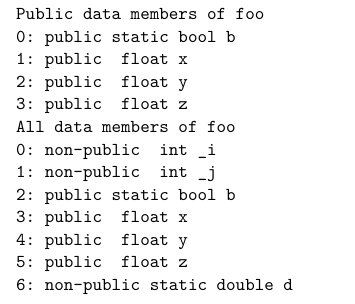
\includegraphics[width=0.8\textwidth]{content/5/chapter8/images/8.png}\\
Displaying the public and private members of the class foo
\end{center}

\subsubsubsection{8.2.3\hspace{0.2cm} Pattern Matching}

New data types such as \href{https://en.cppreference.com/w/cpp/utility/tuple}{std::tuple} or \href{https://en.cppreference.com/w/cpp/utility/variant}{std::variant} need new ways to work with their elements. Simple if or switch conditions or functions like \href{https://en.cppreference.com/w/cpp/utility/apply}{std::apply} or \href{https://en.cppreference.com/w/cpp/utility/variant/visit}{std::visit} can only provide basic functionality. Pattern matching, heavily used in functional programming, enables the more powerful handling of the new data types.

The following code snippets from the proposal \href{http://www.open-std.org/jtc1/sc22/wg21/docs/papers/2020/p1371r2.pdf}{P1371R2} on pattern matching compares classical control structures with pattern matching. Pattern matching uses the keyword inspect and \_\_ for a placeholder.

\begin{itemize}
\item 
switch statement

\hspace*{\fill} \\ %插入空行
\noindent
switch statement versus pattern matching
\begin{lstlisting}[style=styleCXX]
switch (x) {
	case 0: std::cout << "got zero"; break;
	case 1: std::cout << "got one"; break;
	default: std::cout << "don't care";
}

inspect (x) {
	0: std::cout << "got zero";
	1: std::cout << "got one";
	__: std::cout << "don't care";
}
\end{lstlisting}

\item 
if condition

\hspace*{\fill} \\ %插入空行
\noindent
if statement versus pattern matching
\begin{lstlisting}[style=styleCXX]
if (s == "foo") {
	std::cout << "got foo";
} else if (s == "bar") {
	std::cout << "got bar";
} else {
	std::cout << "don't care";
}

inspect (s) {
	"foo": std::cout << "got foo";
	"bar": std::cout << "got bar";
	__: std::cout << "don't care";
}
\end{lstlisting}

The application of pattern matching on std::tuple, std::variant, or polymorphy demonstrates its power.

\item 
std::tuple

\hspace*{\fill} \\ %插入空行
\noindent
std::tuple versus pattern matching
\begin{lstlisting}[style=styleCXX]
auto&& [x, y] = p;
if (x == 0 && y == 0) {
	std::cout << "on origin";
} else if (x == 0) {
	std::cout << "on y-axis";
} else if (y == 0) {
	std::cout << "on x-axis";
} else {
	std::cout << x << ',' << y;
}

inspect (p) {
	[0, 0]: std::cout << "on origin";
	[0, y]: std::cout << "on y-axis";
	[x, 0]: std::cout << "on x-axis";
	[x, y]: std::cout << x << ',' << y;
}
\end{lstlisting}

\item 
std::variant

\hspace*{\fill} \\ %插入空行
\noindent
std::variant versus pattern matching
\begin{lstlisting}[style=styleCXX]
struct visitor {
	void operator()(int i) const {
		os << "got int: " << i;
	}
	void operator()(float f) const {
		os << "got float: " << f;
	}
	std::ostream& os;
};
std::visit(visitor{strm}, v);

inspect (v) {
	<int> i: strm << "got int: " << i;
	<float> f: strm << "got float: " << f;
}
\end{lstlisting}

\item 
Polymorphic data types

\hspace*{\fill} \\ %插入空行
\noindent
Polymorphy versus pattern matching
\begin{lstlisting}[style=styleCXX]
struct Shape { virtual ~Shape() = default; };
struct Circle : Shape { int radius; };
struct Rectangle : Shape { int width, height; };

virtual int Shape::get_area() const = 0;

int Circle::get_area() const override {
	return 3.14 * radius * radius;
}
int Rectangle::get_area() const override {
	return width * height;
}

int get_area(const Shape& shape) {
	return inspect (shape) {
		<Circle> [r] => 3.14 * r * r,
		<Rectangle> [w, h] => w * h
	}
}
\end{lstlisting}
\end{itemize}

The proposal P1371R2 on pattern matching offers more advanced use cases. For example, pattern matching can be used to traverse an \href{https://en.wikipedia.org/wiki/Binary_expression_tree}{expression tree}.








